\documentclass[../../../analisi-dei-requisiti.tex]{subfiles}

\begin{document}

\subsubsection{UUC3: Gestione lista organizzazioni}%
\label{subs:UUC3}

\begin{figure}[H]
  \centering
  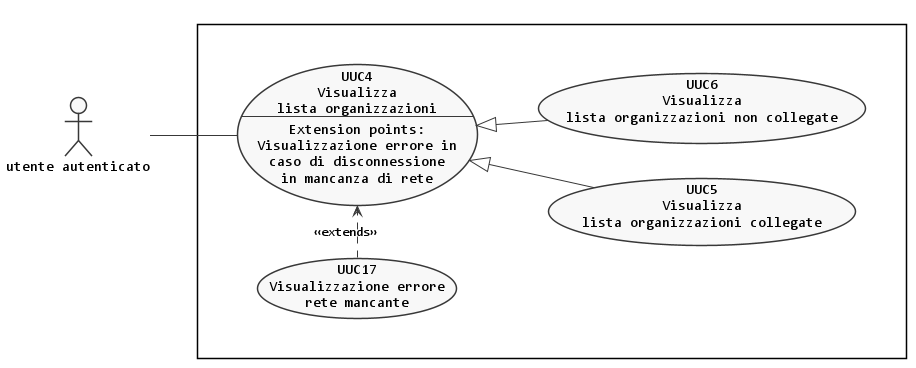
\includegraphics[width=150mm]{gestione-lista-organizzazioni.png}
  \caption{UUC3: Gestione lista organizzazioni}%
  \label{fig:UUC3}
\end{figure}

\begin{description}
  \item[Caso d’uso:] UUC3;
  \item[Titolo:] Gestione lista organizzazioni;
  \item[Attori primari:] utente autenticato;
  \item[Attori secondari:] server LDAP\@;
  \item[Precondizione:] l'utente visualizza la pagina relativa al recupero delle organizzazioni;
  \item[Postcondizione:] l'utente sceglie una o più organizzazioni ed è quindi collegato;
  \item[Scenario principale:]
        \begin{enumerate}
          \item l'utente ha la possibilità di recuperare una lista di organizzazioni alla quale si può collegare;
          \item in caso l'organizzazione alla quale l'utente si vuole collegare sia privata, è richiesta l'autenticazione LDAP all'organizzazione.
        \end{enumerate}
  \item[Estensioni:]
        \begin{enumerate}
          \item in caso di rete mancante, non possono essere eseguite queste operazioni e quindi verrà notificato un errore~\ref{subs:UUC11};
        \end{enumerate}
\end{description}


\subsubsection{UUC3.1: Aggiornamento lista organizzazioni}%
\label{subs:UUC3.1}
\begin{description}
  \item[Caso d’uso:] UUC3.1;
  \item[Titolo:] Aggiornamento lista organizzazioni;
  \item[Attori primari:] utente autenticato;
  \item[Precondizione:] l'utente visualizza la lista delle organizzazioni;
  \item[Postcondizione:] l'utente ha aggiornato la lista delle organizzazioni;
  \item[Scenario principale:]
        \begin{enumerate}
          \item l'utente ha la possibilità di aggiornare la lista delle organizzazioni, e viene avvisato mediante \glossario{notifica} dell'applicazione mobile.
        \end{enumerate}
  \item[Estensioni:]
        \begin{enumerate}
          \item in caso di rete mancante, non può essere eseguito l'aggiornamento della lista di organizzazioni e quindi verrà notificato un errore~\ref{subs:UUC11}.
        \end{enumerate}
\end{description}


\subsubsection{UUC3.2: Scelta organizzazioni}%
\label{subs:UUC3.2}

\begin{figure}[H]
  \centering
  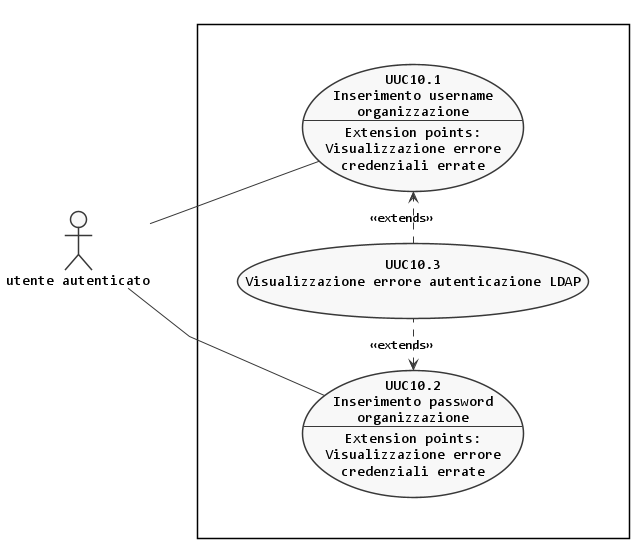
\includegraphics[width=150mm]{autenticazione-ldap-organizzazione.png}
  \caption{UUC3.2: Scelta organizzazioni}%
  \label{fig:UUC3.2}
\end{figure}

\begin{description}
  \item[Caso d’uso:] UUC3.2;
  \item[Titolo:] Scelta organizzazioni;
  \item[Attori primari:] utente autenticato;
  \item[Attori secondari:] server LDAP\@;
  \item[Precondizione:] l'utente visualizza la lista delle organizzazioni alla quale si può collegare;
  \item[Postcondizione:] l'utente ha scelto una o più organizzazioni ed è quindi collegato;
  \item[Scenario principale:]
        \begin{enumerate}
          \item l'utente ha la possibilità di scegliere una o più organizzazioni;
          \item in caso l'organizzazione alla quale l'utente vuole autenticarsi sia privata, è richiesta l'autenticazione tramite il server LDAP, inserendo le credenziali rilasciate dall'organizzazione e univoche per tutti gli utenti interessati ad essere monitorati. In caso contrario, non è richiesta alcuna autenticazione e l'utente si collega direttamente all'organizzazione.
        \end{enumerate}
  \item[Estensioni:]
        \begin{enumerate}
          \item in caso di rete mancante, non possono essere scelte organizzazioni e quindi verrà notificato un errore~\ref{subs:UUC11};
          \item se l'utente si vuole collegare ad un'organizzazione privata e le credenziali inserite dall'utente non corrispondono a quelle dell'organizzazione, allora visualizzerà un errore~\ref{subs:UUC3.2.3}.
        \end{enumerate}
\end{description}

\subsubsection{UUC3.2.1: Inserimento username organizzazione}%
\label{subs:UUC3.2.1}
\begin{description}
  \item[Caso d’uso:] UUC3.2.1;
  \item[Titolo:] Inserimento username organizzazione;
  \item[Attori primari:] utente autenticato;
  \item[Precondizione:] l'utente ha scelto un'organizzazione privata e non ha ancora inserito lo username dell'organizzazione;
  \item[Postcondizione:] l'utente ha inserito lo username dell'organizzazione privata;
  \item[Scenario principale:]
        \begin{enumerate}
          \item l'utente inserisce lo username relativo all'organizzazione privata alla quale vuole collegarsi;
        \end{enumerate}
  \item[Estensioni:]
        \begin{enumerate}
          \item se lo username inserito dall'utente non corrisponde a quello dell'organizzazione privata, allora visualizzerà un errore~\ref{subs:UUC3.2.3}.
        \end{enumerate}
\end{description}

\subsubsection{UUC3.2.2: Inserimento password organizzazione}%
\label{subs:UUC3.2.2}
\begin{description}
  \item[Caso d’uso:] UUC3.2.2;
  \item[Titolo:] Inserimento password organizzazione;
  \item[Attori primari:] utente autenticato;
  \item[Precondizione:] l'utente ha scelto un'organizzazione privata e non ha ancora inserito la password dell'organizzazione;
  \item[Postcondizione:] l'utente ha inserito la password dell'organizzazione privata;
  \item[Scenario principale:]
        \begin{enumerate}
          \item l'utente inserisce la password relativa all'organizzazione privata alla quale vuole collegarsi;
        \end{enumerate}
  \item[Estensioni:]
        \begin{enumerate}
          \item se la password inserita dall'utente non corrisponde a quella dell'organizzazione privata, allora visualizzerà un errore~\ref{subs:UUC3.2.3}.
        \end{enumerate}
\end{description}

\subsubsection{UUC3.2.3: Visualizzazione errore autenticazione LDAP}%
\label{subs:UUC3.2.3}
\begin{description}
  \item[Caso d’uso:] UUC3.2.3;
  \item[Titolo:] Visualizzazione errore autenticazione LDAP\@;
  \item[Attori primari:] utente autenticato;
  \item[Precondizione:] i dati forniti dall'utente non corrispondono a credenziali valide;
  \item[Postcondizione:] l'applicazione mobile comunica all'utente il fallimento dell'autenticazione;
  \item[Scenario principale:]
        \begin{enumerate}
          \item l'utente cerca di effettuare l'autenticazione LDAP all'organizzazione privata con credenziali errate.
        \end{enumerate}
\end{description}

\end{document}
